\documentclass[aspectratio=169]{beamer}
% Shared preamble for ml/ slide decks.
% Each lecture .tex starts with:
%   \documentclass[aspectratio=169]{beamer}
%   \input{../preamble}
% Compile from inside the chapter folder so \input{../preamble} resolves.

\usetheme{default}
\usecolortheme{dove}

\setbeamertemplate{navigation symbols}{}
\setbeamertemplate{footline}{%
  \hfill{\large\insertframenumber\,/\,\inserttotalframenumber}\hspace{0.8em}\vspace{0.5em}%
}

% Project palette (existing, kept for backwards compatibility with deferred/*)
\definecolor{popblue}{RGB}{52, 101, 164}
\definecolor{sampred}{RGB}{204, 0, 0}
\definecolor{paramgreen}{RGB}{0, 140, 70}
\definecolor{warnred}{RGB}{180, 40, 40}
\definecolor{orange1}{RGB}{220, 120, 0}
\definecolor{violet1}{RGB}{120, 50, 160}
\definecolor{lightbg}{RGB}{245, 245, 250}

% Armenian flag palette (use these for any 3-color highlight; per CLAUDE.md).
% "Nice versions": slightly de-saturated from the official spec for slide use,
% so they don't burn out under projector colors. Originals kept as *_pure.
\definecolor{armred}{RGB}{200, 30, 40}      % nice red (official #D90012 muted)
\definecolor{armblue}{RGB}{30, 70, 160}     % nice blue (official #0033A0 muted)
\definecolor{armorange}{RGB}{230, 160, 30}  % nice orange (official #F2A800 muted)
\definecolor{armred_pure}{HTML}{D90012}     % official Armenian flag red
\definecolor{armblue_pure}{HTML}{0033A0}    % official Armenian flag blue
\definecolor{armorange_pure}{HTML}{F2A800}  % official Armenian flag orange

\setbeamercolor{frametitle}{fg=popblue}
\setbeamercolor{title}{fg=popblue}

\usepackage{pgfplots}
\usepackage{tikz}
\usetikzlibrary{shapes, arrows.meta, positioning, calc, decorations.pathreplacing, patterns, matrix}
\pgfplotsset{compat=1.18}
\usepackage{amsmath, amssymb, amsfonts}
\usepackage{bm}
\usepackage{dsfont}
\usepackage{array}
\usepackage{pifont}
\usepackage{colortbl}
\usepackage{fontenc}

% Callout boxes. Purely additive - existing decks are unaffected.
% Usage: \begin{tcolorbox}[colback=armblue!8, colframe=armblue, boxrule=0.6pt, arc=2pt,
%                          title=\textbf{Key idea}] ... \end{tcolorbox}
% Palette convention (ml/SLIDE_STYLE.md): armblue=key idea, armred=trap/warning,
% paramgreen=takeaway or "Next", armorange=watch-out.
\usepackage[most]{tcolorbox}

% Cleaner table rules (\toprule, \midrule, \bottomrule). Also purely additive.
\usepackage{booktabs}

% \cancel{...} for struck-through terms in derivations (added 2026-08-11 for the
% importance-sampling frame in ch11_rl, where the dynamics cancel). Purely additive.
\usepackage{cancel}

% Minimal ML notation macros (subset of slds-lmu latex-math/basic-ml.tex).
% Kept here so we don't have to inline-expand every \thetav, \xv, etc.
% when porting upstream slides.
\newcommand{\R}{\mathds{R}}
\newcommand{\N}{\mathds{N}}
\newcommand{\E}{\mathds{E}}
\newcommand{\Xspace}{\mathcal{X}}
\newcommand{\Yspace}{\mathcal{Y}}
\newcommand{\Hspace}{\mathcal{H}}
\newcommand{\D}{\mathcal{D}}
\newcommand{\Dtrain}{\mathcal{D}_{\text{train}}}
\newcommand{\Dtest}{\mathcal{D}_{\text{test}}}
\newcommand{\xv}{\mathbf{x}}
\newcommand{\yv}{\mathbf{y}}
\newcommand{\Xmat}{\mathbf{X}}
\newcommand{\id}{\mathbf{I}}
\newcommand{\thetav}{\bm{\theta}}
\newcommand{\thetah}{\hat{\bm{\theta}}}
\newcommand{\lamv}{\bm{\lambda}}
\newcommand{\fx}{f(\xv)}
\newcommand{\fxt}{f(\xv \,|\, \bm{\theta})}
\newcommand{\fxi}{f\!\left(\xv^{(i)}\right)}
\newcommand{\fh}{\hat{f}}
\newcommand{\fxh}{\hat{f}(\xv)}
\newcommand{\yh}{\hat{y}}
\newcommand{\yih}{\hat{y}^{(i)}}
% \xi clashes with the Greek letter \xi; write \xv^{(i)} inline instead.
\newcommand{\yi}[1][i]{y^{(#1)}}
\newcommand{\xyi}[1][i]{\left(\xv^{(#1)},\, y^{(#1)}\right)}
\newcommand{\thx}{\bm{\theta}^\top \xv}
\newcommand{\sumin}{\sum_{i=1}^{n}}
\newcommand{\sumjp}{\sum_{j=1}^{p}}
\newcommand{\Lxy}{L\!\left(y, \fx\right)}
\newcommand{\Lxyi}{L\!\left(\yi, \fxi\right)}
\newcommand{\risk}{\mathcal{R}}
\newcommand{\riske}{\mathcal{R}_{\text{emp}}}
\newcommand{\risket}{\mathcal{R}_{\text{emp}}(\bm{\theta})}
\newcommand{\riskt}{\mathcal{R}(\bm{\theta})}
\newcommand{\riskr}{\mathcal{R}_{\text{reg}}}
\newcommand{\argmin}{\mathop{\mathrm{arg\,min}}}
\newcommand{\argmax}{\mathop{\mathrm{arg\,max}}}
\newcommand{\eps}{\varepsilon}


\graphicspath{{fig/}{../00_shared/fig/}}

% callout boxes, matching the chapter's fcolorbox house pattern (LLM-1 to LLM-13)
\newcommand{\keybox}[1]{\fcolorbox{armblue}{armblue!8}{\parbox{0.97\linewidth}{\small #1}}}
\newcommand{\trapbox}[1]{\fcolorbox{armred}{armred!8}{\parbox{0.97\linewidth}{\small #1}}}
\newcommand{\takebox}[1]{\fcolorbox{paramgreen}{paramgreen!8}{\parbox{0.97\linewidth}{\small #1}}}
\newcommand{\watchbox}[1]{\fcolorbox{armorange}{armorange!12}{\parbox{0.97\linewidth}{\small #1}}}

\newcommand{\sectiontransition}[2]{%
  \begin{frame}[plain]
    \vfill
    \begin{center}
      {\Huge\bfseries\color{popblue} #1}\\[1.1em]
      {\large #2}
    \end{center}
    \vfill
  \end{frame}}

\newcommand{\src}[1]{{\scriptsize\color{gray} #1}}

\title{Anatomy of a 2026 LLM}
\subtitle{What changed since GPT-2, and what each change saves}
\author{}
\date{}

\begin{document}

\begin{frame}[plain]
  \titlepage
  \begin{center}\scriptsize\color{gray}
    LLM chapter, session 14. Model facts from published configuration files, read 2026-10-06.
  \end{center}
\end{frame}

% ============================================================ WHERE WE ARE (py_src/llm_roadmap.py)
\begin{frame}{Where we are: one forward pass}
  \begin{center}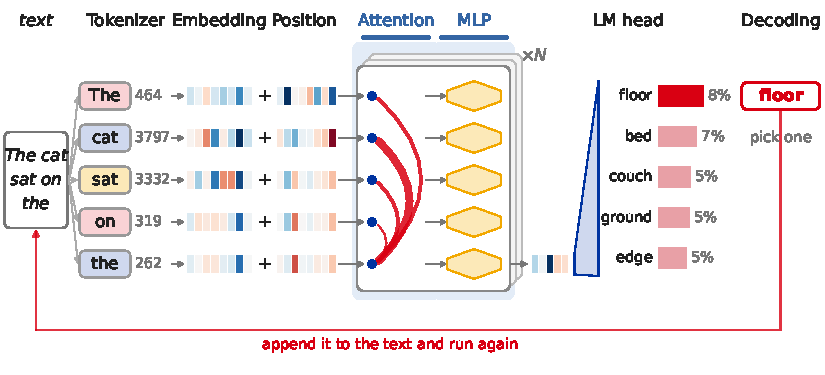
\includegraphics[width=\linewidth]{roadmap_anatomy_2026_pass.pdf}\end{center}
  \vskip -2pt
  {\small Every box is still there. Today: what 2026 models changed inside them.}
\end{frame}

\begin{frame}{Where we are: the life of a model}
  \begin{center}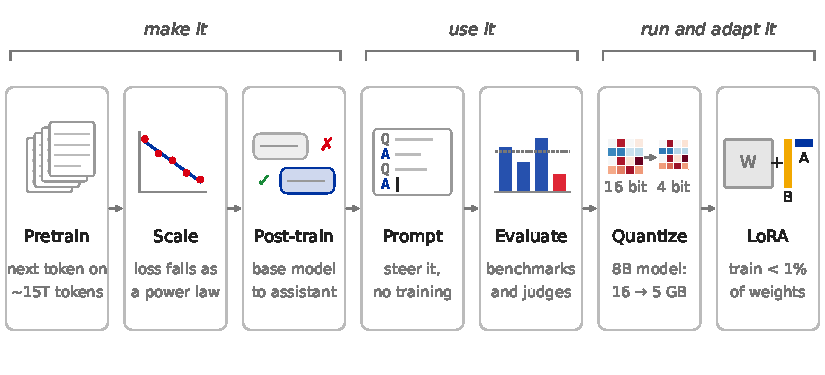
\includegraphics[width=\linewidth]{roadmap_anatomy_2026_life.pdf}\end{center}
  \vskip -2pt
  {\small The last lecture of the chapter: the whole life, seen through one modern model.}
\end{frame}

% ============================================================ COLD OPEN
\begin{frame}{Two configuration files}
  \vskip 2pt
  \begin{center}
  \small
  \begin{tabular}{lcc}
    \toprule
    & \textbf{GPT-2 small (2019)} & \textbf{gpt-oss-20b (2025)} \\
    \midrule
    layers & 12 & 24 \\
    attention heads (size) & 12 (64) & 64 (64) \\
    key/value heads & 12 & \textbf{8} \\
    attention span & every layer: all tokens & \textbf{every other layer: last 128} \\
    feed-forward & one MLP & \textbf{32 experts, 4 used per token} \\
    parameters & 124M & 21B stored, \textbf{3.6B used per token} \\
    context & 1,024 & 131,072 \\
    \bottomrule
  \end{tabular}
  \end{center}

  \vskip 8pt
  \trapbox{\textbf{Predict first:} the bold entries are the new ideas (each one is explained today;
  for now, guess from the words). What do they have in common?}
\end{frame}

\begin{frame}{They all save memory or compute when the model runs}
  \vskip 2pt
  {\small \textbf{Answer}: each one makes the model cheaper to run.}
  \vskip 2pt
  \begin{itemize}
    \item \textbf{8 key/value heads, not 64}: groups of 8 query heads share one key and one value,
      so the KV cache (LLM-12) is 8$\times$ smaller. Section ``The KV cache''.
    \item \textbf{A 128-token window in half the layers}: those layers look only at the last 128
      tokens, so their cache stops growing. Same section.
    \item \textbf{Experts}: many feed-forward parts, of which each token uses 4: 21B parameters of
      knowledge, 3.6B of work per token. Section ``Compute and traffic''.
  \end{itemize}

  \vskip 6pt
  {\small The block of LLM-4 is still recognisable: residual stream, attention, a feed-forward
  part, normalisation. What changed is mostly \emph{how much each part costs to run}.}

  \vskip 6pt
  \keybox{Training happens once; a model answers billions of times. So almost every change since
  2019 is a way to pay less per token. Today: each one with its bill, from a real config.}
\end{frame}

\begin{frame}{Outline}
  \tableofcontents
\end{frame}

% ============================================================ 1. THE KV CACHE
\section{The KV cache}
\sectiontransition{The KV cache}{Long contexts are expensive. Here is why, and the fixes.}

\begin{frame}{Prefill and decode}
  \vskip 6pt
  \begin{itemize}
    \item \textbf{Prefill}: the whole prompt goes through in one pass, all positions in parallel
      (LLM-4). Big matrix multiplications: limited by arithmetic.
    \item \textbf{Decode}: one new token per pass. Each pass reads all the weights \emph{and} the KV
      cache of every earlier token: limited by memory bandwidth (LLM-12).
    \item The KV cache grows with every token (LLM-12). Bytes per token: $2_{\,\text{K,V}} \times
      \text{layers} \times \text{KV heads} \times \text{head size} \times 2_{\,\text{bytes}}$ -
      one 2 for keys and values, one for 16-bit numbers.
  \end{itemize}

  \vskip 10pt
  \keybox{Every byte of cache per token is read again for every new token. Shrinking it makes long
  conversations both fit and run faster.}
\end{frame}

\begin{frame}{Fewer key/value heads}
  \vskip 4pt
  \begin{itemize}
    \item \textbf{Multi-head} (LLM-3): every query head has its own keys and values.
    \item \textbf{Multi-query} (MQA): all query heads share \emph{one} key/value head.
    \item \textbf{Grouped-query} (GQA): query heads share in groups - Llama 3 8B: 32 query heads in
      8 groups of 4, each group sharing one key head and one value head.
  \end{itemize}

  \vskip 6pt
  \textbf{By hand}, bytes per token (16-bit):
  \vskip 2pt
  \begin{center}
  \footnotesize
  \begin{tabular}{lrr}
    \toprule
    & \textbf{as built} & \textbf{if multi-head} \\
    \midrule
    Falcon-7B (MQA: 1 of 71) & $2 \times 32 \times 1 \times 64 \times 2 = 8{,}192$ & 581,632 (71$\times$) \\
    Llama 3 8B (GQA: 8 of 32) & $2 \times 32 \times 8 \times 128 \times 2 = 131{,}072$ & 524,288 (4$\times$) \\
    \bottomrule
  \end{tabular}
  \end{center}
  \vskip 4pt
  {\small One shared head saves the most and costs some quality; GQA is the compromise most current
  models chose (gpt-oss: 8).}
\end{frame}

\begin{frame}{Cache a compressed version: MLA}
  \begin{columns}[c]
    \column{0.58\textwidth}
      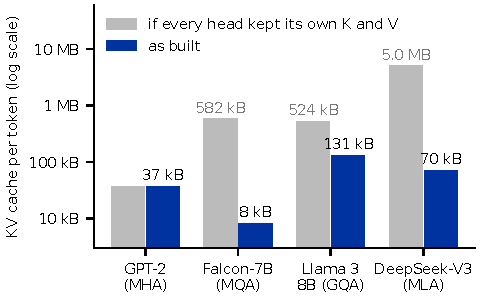
\includegraphics[width=\linewidth]{anat_kv.pdf}
    \column{0.40\textwidth}
      {\small \textbf{Multi-head latent attention} (DeepSeek): per layer and token, cache one
      \emph{latent} vector - a compressed summary the model learns to make. Every head's keys and
      values are rebuilt from it when needed.

      \vskip 6pt
      \textbf{The bill}: extra matrix multiplications for the rebuild. Decode waits on memory,
      not arithmetic (LLM-12), so it is a good trade.}
  \end{columns}
\end{frame}

\begin{frame}{MLA by hand: DeepSeek-V3}
  \vskip 4pt
  \begin{itemize}
    \item \textbf{As built}, per layer: a 512-number latent plus a 64-number key part that carries
      the position (RoPE, LLM-2). $576 \times 2_{\,\text{bytes}} \times 61$ layers $= 70{,}272$
      bytes per token. No $2_{\,\text{K,V}}$: keys and values both come from the one vector.
    \item \textbf{If multi-head}: 128 heads, each with a key of $128 + 64 = 192$ numbers and a value
      of 128. $128 \times (192 + 128) \times 2_{\,\text{bytes}} \times 61 = 4{,}997{,}120$ bytes,
      about 5.0 MB per token.
    \item Ratio: 71$\times$. Falcon's MQA also saved 71$\times$, by coincidence: 71 heads there,
      a 576-number vector against 128 heads of 320 numbers here.
  \end{itemize}

  \vskip 8pt
  \keybox{At 128K tokens: 9.2 GB of cache instead of 655 GB. Without MLA, one long conversation's
  cache would be about as big as the whole model's 671B weights in 8-bit.}
  \vskip 2pt
  \src{Config: DeepSeek-V3 (kv\_lora\_rank 512, qk\_rope\_head\_dim 64, qk\_nope\_head\_dim 128,
  v\_head\_dim 128, 61 layers).}
\end{frame}

\begin{frame}{Look back less: sliding windows}
  \vskip 6pt
  \begin{itemize}
    \item A \textbf{sliding-window} layer attends only to the last $w$ tokens, so its cache stops
      growing at $w$.
    \item gpt-oss-20b alternates: 12 layers with a 128-token window, 12 layers with full attention.
      The full layers keep the long-range view.
    \item \textbf{By hand}, per layer and token: $2_{\,\text{K,V}} \times 8 \text{ KV heads} \times 64
      \times 2_{\,\text{bytes}} = 2{,}048$ bytes. At 128K tokens, all 24 layers full: $24 \times
      2{,}048 \times 131{,}072 = 6.4$ GB. Alternating: the 12 windowed layers hold only 128 tokens
      each, so about 3.2 GB.
  \end{itemize}

  \vskip 8pt
  \watchbox{Half the cache, but not for free: a windowed layer loses direct access to old tokens.
  The full layers in between carry the long-range information. That trade is a design choice,
  tested on benchmarks.}
\end{frame}

\begin{frame}{Or a fixed-size memory: linear attention}
  \vskip 6pt
  \begin{itemize}
    \item Some layers replace attention with a \textbf{linear-attention} layer that keeps a
      fixed-size state, updated token by token - an RNN's memory (L21's ``recurrence comeback'').
    \item Qwen3-Next-80B-A3B: 48 layers, full attention in every 4th layer only (12 of 48). Only
      those keep a growing cache: $2_{\,\text{K,V}} \times 12 \text{ layers} \times 2 \text{ KV
      heads} \times 256 \times 2_{\,\text{bytes}} = 24{,}576$ bytes per token. The linear layers'
      fixed-size state comes on top, but it does not grow with the context.
    \item The cost: a fixed-size state forgets; the full-attention layers in between recall exactly.
  \end{itemize}

  \vskip 10pt
  \keybox{Four answers to one bill: share heads (GQA), compress (MLA), look back less (windows),
  remember in fixed size (linear attention). Real 2026 models mix them.}
\end{frame}

% ============================================================ 2. COMPUTE
\section{Compute and traffic}
\sectiontransition{Compute and traffic}{Big knowledge, small work per token, fewer trips to memory.}

\begin{frame}{Mixture of experts}
  \begin{columns}[c]
    \column{0.58\textwidth}
      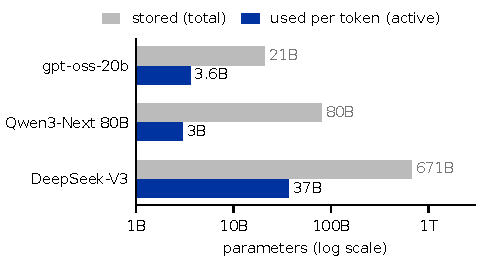
\includegraphics[width=\linewidth]{anat_moe.pdf}
    \column{0.40\textwidth}
      {\small Replace the one feed-forward MLP with many smaller ones, the \textbf{experts}. A small
      \textbf{router} scores them for each token and sends the token to the top few.

      \vskip 4pt
      gpt-oss-20b: 32 experts, 4 per token. Qwen3-Next: 512, 10 per token. DeepSeek-V3: 256 routed,
      8 per token, plus 1 \textbf{shared} expert that every token uses.}
  \end{columns}

  \vskip 6pt
  \keybox{DeepSeek-V3 stores 671B parameters and uses 37B per token: it stores 18$\times$ more
  than it uses. MoE buys a big model's knowledge at a small model's cost per token, and pays in
  memory.}
\end{frame}

\begin{frame}{MoE by hand: what is saved, and when}
  \vskip 4pt
  \begin{itemize}
    \item \textbf{Arithmetic}: a forward pass costs about 2 FLOPs per \emph{active} parameter
      (LLM-8). gpt-oss-20b: about 7 GFLOPs per token, against 42 if all 21B were used.
    \item \textbf{Memory traffic}, with one user: each token reads only the weights it uses (3.6B of
      21B), so decode, which waits on memory, speeds up too.
    \item \textbf{In a big batch} (``Serving many users''): different tokens pick different experts, so most
      experts get read anyway. The saving is then in arithmetic only.
  \end{itemize}

  \vskip 8pt
  \watchbox{Memory must hold all 21B either way (or 4-bit, LLM-12). MoE saves work per token, not
  space.}
\end{frame}

\begin{frame}{Keeping the experts busy}
  \vskip 6pt
  \begin{itemize}
    \item A router left alone sends most tokens to a few favourite experts; the rest never learn,
      and the favourites become a bottleneck.
    \item The usual fix is an extra loss that rewards balanced use. DeepSeek-V3 instead adjusts a
      per-expert bias during training (``auxiliary-loss-free'').
    \item \textbf{Shared experts} (DeepSeek-V3 has one): they learn what all tokens need, so the
      routed experts can specialise.
  \end{itemize}

  \vskip 10pt
  \watchbox{Experts are not ``the maths expert'' and ``the history expert''. They specialise in
  patterns the router finds useful, which rarely match human topics.}
\end{frame}

\begin{frame}{FlashAttention: the same numbers, fewer trips}
  \vskip 6pt
  \begin{itemize}
    \item The attention bill was quadratic (LLM-5). In training and prefill the full $n \times n$
      score matrix exists, and on a GPU the slow part is often moving it to and from memory, not
      computing it. (In decode the scores are a single row.)
    \item A GPU has a little fast memory on the chip (SRAM) and a lot of slower main memory (HBM).
      On an A100, SRAM has about 10$\times$ HBM's bandwidth and is about 2000$\times$ smaller.
    \item FlashAttention (Dao et al., 2022) works through small blocks (tiles) of queries and keys
      that fit in the fast memory, and never writes the full $n \times n$ matrix to main memory.
  \end{itemize}

  \vskip 8pt
  \takebox{Exact, not an approximation: the same outputs and about the same arithmetic, much less
  memory traffic. A big part of why long contexts became practical to train.}
\end{frame}

\begin{frame}{More than one token per step}
  \vskip 6pt
  \begin{itemize}
    \item Decoding writes one token per pass. LLM-6's \textbf{speculative decoding}: a small draft
      model guesses several tokens, the big model checks them in one pass, and the output stays
      exactly the big model's.
    \item \textbf{Multi-token prediction}: DeepSeek-V3 adds one extra Transformer block that takes
      the main model's hidden state and predicts the token \emph{after} next. It shares the main
      model's embedding and output head. It helps training, and at inference it serves as the draft.
    \item Measured by DeepSeek: the drafted second token is accepted 85-90\% of the time, for
      1.8$\times$ the tokens per second.
  \end{itemize}

  \vskip 10pt
  \keybox{Both turn the bandwidth-bound decode into fewer, fuller passes.}
\end{frame}

% ============================================================ 3. SERVING
\section{Serving many users}
\sectiontransition{Serving many users}{The same tricks, at scale.}

\begin{frame}{Batching: shared weights, private caches}
  \vskip 6pt
  \begin{itemize}
    \item One user leaves the GPU mostly idle (decode is bandwidth-bound). Batching many users
      reads the weights once per step for all of them. But each user has their own KV cache.
    \item \textbf{By hand}, Llama 3 8B: the weights, $8\text{B} \times 2_{\,\text{bytes}} = 16$ GB,
      shared. One user at 4,096 tokens: $131{,}072 \times 4{,}096 \approx 0.54$ GB of cache. About
      30 such users need as much memory for caches as for the weights.
    \item \textbf{Continuous batching}: requests join and leave the batch at every step, instead of
      waiting for the slowest one to finish.
  \end{itemize}

  \vskip 8pt
  \keybox{With many users, the caches, not the weights, fill the GPU. So serving is mostly about
  cache memory.}
\end{frame}

\begin{frame}{PagedAttention: cache memory in pages}
  \vskip 6pt
  \begin{itemize}
    \item Without it, each request reserves one big block of cache memory, sized for the longest
      answer it might give. Much of that block stays empty.
    \item \textbf{PagedAttention} (Kwon et al., 2023, vLLM): store each request's cache in small
      fixed-size pages, the way an operating system hands out memory. A request that needs 3 pages
      gets any 3 free pages, and more as it grows.
    \item Near-zero wasted cache memory, so more users fit in a batch: 2-4$\times$ the throughput of
      earlier serving systems (FasterTransformer, Orca) at the same latency.
  \end{itemize}

  \vskip 8pt
  {\small These are the server engines of LLM-12. On a laptop, with one user, they matter less.}
\end{frame}

% ============================================================ 4. WHAT DID NOT CHANGE
\section{What did not change}
\sectiontransition{What did not change}{The 2017 core.}

\begin{frame}{What did not change}
  \vskip 6pt
  \begin{itemize}
    \item The residual stream with attention and feed-forward parts added to it (LLM-4).
    \item Next-token pretraining on filtered web text (LLM-7), then post-training (LLM-9).
    \item Tokens, embeddings, a softmax over the vocabulary at the end (LLM-1, LLM-2, LLM-5).
  \end{itemize}

  \vskip 10pt
  \keybox{A student of 2017's Transformer can read a 2026 configuration file. Most of the new
  words in it - GQA, MLA, sliding window, experts - name a way to make the same computation
  cheaper to run.}
\end{frame}

% ============================================================ CLOSE
\begin{frame}{Recap}
  \small
  \begin{itemize}
    \item \textbf{Inference cost drives the design}: decode is bandwidth-bound, and the KV cache
      grows with every token.
    \item \textbf{Smaller cache}: GQA (Llama 3 8B, 4$\times$), MQA (Falcon-7B, 71$\times$), MLA
      (DeepSeek-V3, also 71$\times$), sliding windows (gpt-oss: half), linear-attention layers
      (Qwen3-Next: 1 in 4 full).
    \item \textbf{Less work and traffic}: MoE (gpt-oss-20b: 3.6B of 21B per token), FlashAttention
      (fewer memory trips), multi-token prediction (1.8$\times$ tokens per second) and speculative
      decoding.
    \item \textbf{Serving}: shared weights, private caches - continuous batching and paged KV memory.
    \item \textbf{Unchanged}: the residual stream, attention, next-token training.
  \end{itemize}
\end{frame}

\begin{frame}{The end of the map}
  \begin{center}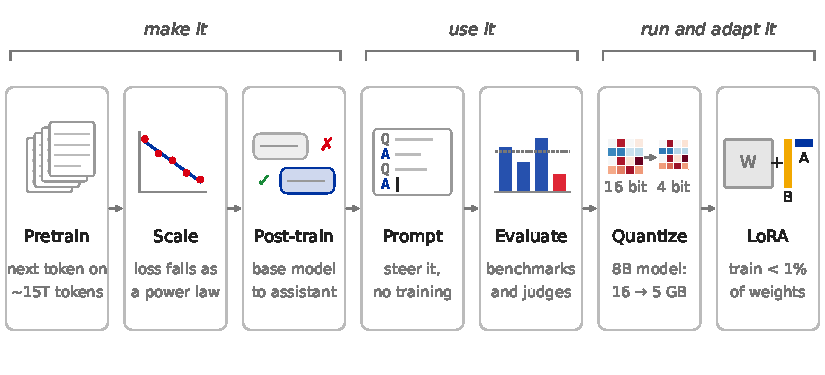
\includegraphics[width=\linewidth]{roadmap_overview_life.pdf}\end{center}
  \vskip -2pt
  {\small The whole chapter: tokens to a 2026 model.}
\end{frame}

\begin{frame}{Sources \& further reading}
  \footnotesize
  \begin{itemize}
    \item Configuration files (Hugging Face, read 2026-10-06): openai/gpt-oss-20b,
      deepseek-ai/DeepSeek-V3, tiiuae/falcon-7b, Qwen/Qwen3-Next-80B-A3B-Instruct; Llama 3 paper,
      Table 3.
    \item Shazeer (2019), multi-query attention; Ainslie et al. (2023), GQA; DeepSeek-AI (2024),
      DeepSeek-V2 and V3 (MLA, MoE, multi-token prediction).
    \item Dao et al. (2022), ``FlashAttention''; Kwon et al. (2023), ``Efficient Memory Management
      for Large Language Model Serving with PagedAttention''.
  \end{itemize}
  \vskip 2pt
  \src{Figures: \texttt{py\_src/anatomy\_figs.py}. Every number computed by hand from the configs
  above and asserted there.}
\end{frame}

\end{document}

% ============================================================================
% Provenance:
%   Deck: LLM-14 Anatomy of a 2026 LLM (14_llms), session 14. Built 2026-10-06 from the critique in
%   LLM_CHAPTER_PLAN.md (LLM-14) and the queue (instructor: "do all queue items"; D1 answered - no
%   session limit, LLM-14 built, one deck unless it outgrows it: DECISIONS #73), with the
%   recommended "each technique with its bill by hand from one real config".
%   Configs fetched 2026-10-06 from Hugging Face config.json files (gpt-oss-20b, DeepSeek-V3,
%   Falcon-7B, Qwen3-Next-80B-A3B-Instruct); Llama 3 8B from the paper's Table 3 (local deck).
%   Other facts: DeepSeek-V3 671B / 37B and its MTP and auxiliary-loss-free balancing
%   (sources/llm_training/17_deepseek_v3); FlashAttention's SRAM vs HBM numbers on an A100
%   (sources/llm_training/15_flash_attention); PagedAttention's abstract (fetched).
%   MTP's 85-90% acceptance and 1.8x tokens per second: DeepSeek-V3 paper, section 5.4.3
%   (ml/llm_training/materials_md/papers/23_deepseek_v3_2412.19437.txt).
%   Every printed number is asserted in py_src/anatomy_figs.py; sizes use decimal units (kB, MB, GB)
%   throughout, so every ratio recomputes exactly.
%   Student review (one Sonnet agent, 2026-10-06) applied: GiB vs GB mixed on the MLA frame (now
%   decimal), the two factors of 2 tagged (K,V and bytes), the coincidental 71x named, MLA split
%   into idea + by-hand frames with its bill, "for free" on windows removed, MoE split with the
%   bandwidth vs FLOPs caveat and 37B shown, FlashAttention placed in prefill/training, MTP's
%   measured speedup, serving split with a by-hand cache count, terms glossed where first used.
%   Cut (plan): RoPE and long-context extension (LLM-2), the dated landscape list (perishable),
%   diffusion LMs (a forward pointer would need the diffusion chapter's order), attention sinks
%   (not in gpt-oss-20b's config; unverified here).
% ============================================================================
